\documentclass{article}
\usepackage[utf8]{inputenc}

\title{Convolution in OpenCl}
\author{Group 1: Jeremy Lang, Reuben Speirs, Victor Startsev}
\date{June 2020}

\usepackage{graphicx}
\usepackage{todonotes}

\begin{document}

\maketitle

\section{Introduction}

Often times applications that process digital signals need to be able to filter input data, in order to remove noise for example, before the application can perform further analysis. Our project was to design an application that implements a finite impulse response (FIR) filter. FIR filtering is one of the most common techniques employed to filter digital signals. Our FIR was to take in a one-dimensional (1-D) array of size M, which is an array of signal data, and another 1-D array of size N, an array of tap coefficients for the FIR. 

To achieve parallelisation results we use the OpenCL library. It is a framework for writing programs that take advantage of hardware acceleration but without limiting the programs to one form of hardware acceleration such has using NVIDIA CUDA would. The general purpose is to launch work items that are run on the accelerator and read the results on a host system. This project uses OpenCL to launch kernels that perform the core operations of an FIR filter.

As part of the requirements for this project, we are to use OpenCL to perform the convolution between the two arrays on a graphics card (GPU). This is because for relatively short data, implementing an FIR filter is trivial. However, when the data that needs to be processed is relatively large, the application needs to be able to break the input data into chunks and process each chunk in parallel, in order to increase efficiency. In order to process chunks independently, an acceleration unit, like a GPU or an FPGA, can be sent chunks of data that need to be processed. Acceleration units are designed to be able to perform math operations efficiently and in parallel, making them ideal for our situation.

\section{Implementation}

\subsection{Matlab implementation}

Matlab is a powerful math modelling and analysis programming language/tool that is widely used in the engineering, science and economics disciplines. We have decided to use this tool because it allows us to quickly generate data that we can output to a “.csv” file that can then be used by our C++ implementation. Additionally, Matlab allows us to graph the data we plan to send to our C++ implementation, graph the expected output, and to view the output of our C++ implementation. By comparing the results generated by our C++ implementation and what we have in Matlab we are able to validate that our implementation is correct.

\begin{figure}[!htb]
	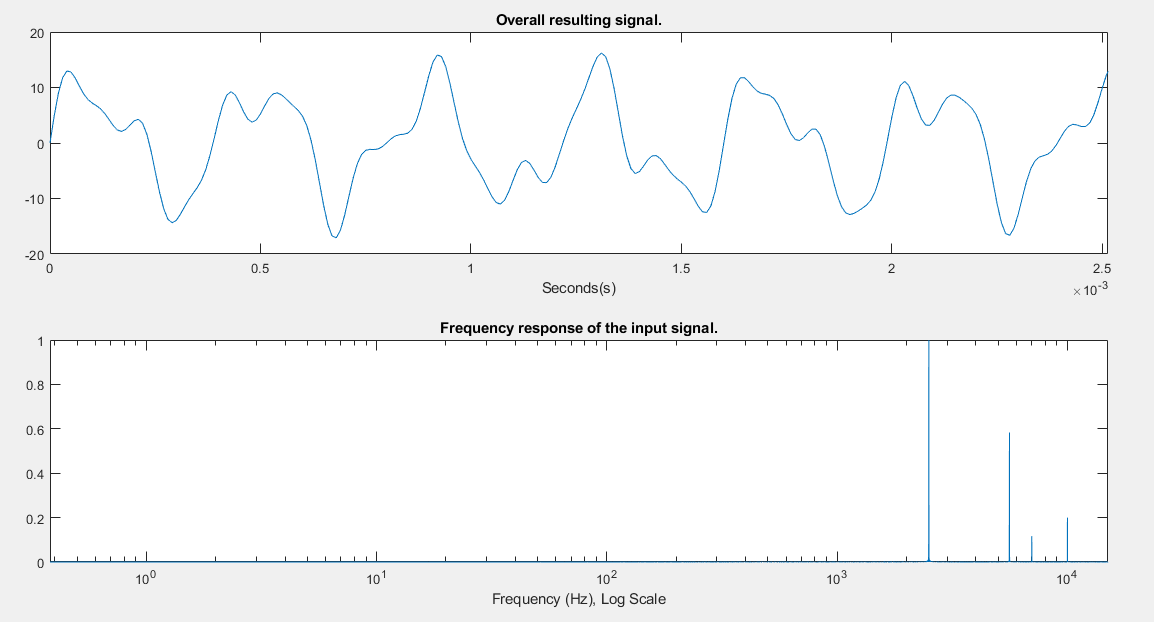
\includegraphics[width=\linewidth]{matlab1.png}
	\caption{A) The graph at the top is the overall waveform that is produced by “FIR.m”. B) The graph at the bottom is the frequency component of the overall wave.}
	\label{fig:mat1}
\end{figure}

In our project, under \begin{verbatim}project\Matlab\MATLAB FIR filter\\end{verbatim} there is a file known as “FIR.m”. This Matlab script completes four functions. First, it generates a set of waves at different frequencies by using the generic wave equation yx = A*sin(2*pi*fx*t) and some sample times. We then add together the waves to produce a resultant waveform (Fig 1.A.). Next, the script generates a set of coefficients for an FIR filter that satisfies a given order and cutoff frequency(/s) (Fig. 2.B.). FIR coefficient, the sample times and the y-value of the overall signal are then outputted to a csv that will be used by our C++ implementation. Afterwards, both the FIR filter coefficients and the resultant waveform (Fig. 1.B.) are converted into the frequency domain using a fast fourier transform function (FFT) (Fig. 2.B.). Lastly, the waveform and filter, in the frequency domain, are multiplied together and their result is passed to an inverse FFT function to get a convolution between the FIR filter and an input waveform as a result. From this we get a waveform that has some of its frequency components removed (Fig. 2.C.). We then use the figure generated by this code (Fig. 2.) as a ground truth comparison for our C++ implementation.


\begin{figure}[!htb]
	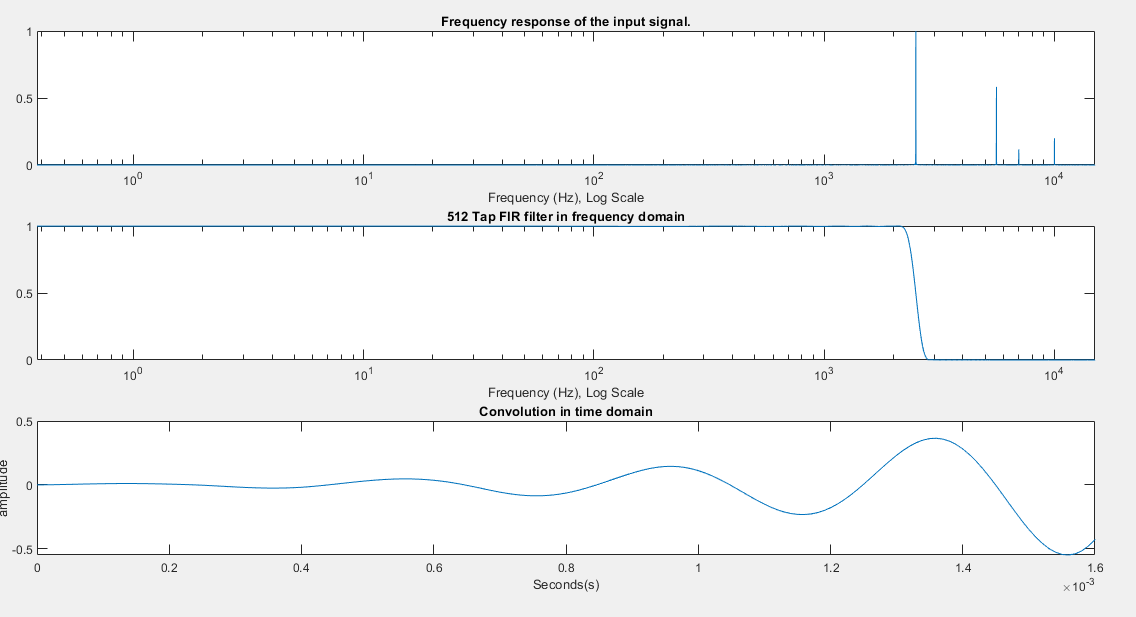
\includegraphics[width=\linewidth]{matlab2.png}
	\caption{A) The top graph is the frequency component of our resultant wave. B) The middle graph is the result of transferring our FIR coefficients into the frequency domain. C) The bottom graph represents our expected output, i.e. the filtered wave.}
	\label{fig:mat2}
\end{figure}

.

\subsection{Reading and writing CSV, file I/O decisions}

Because the size of the RAM is limited we need to store the input data into our C++ implementation on disk as a csv file. By having all of our data on disk, our implementation suffers from an input bottleneck. This is because reading data that is stored on the disk is an expensive operation, as disk access times are typically much slower than cache or RAM access times. 

In order to minimise the effect of having to read from the disk we load our file into virtual memory using the \begin{verbatim}mapped_file_source\end{verbatim} class provided in the boost library. By mapping the entirety of our file into a virtual address space we are able to get back some of the benefits of using RAM. When the file is mapped, boost will provide us with a page from our csv file that will be loaded into RAM. However, eventually we will reach the end of the loaded page and the application will have to go back into disk to grab the next page in our csv file, meaning we will need to read from the disk to get the next page of data. The new page will be put into RAM. Effectively this reduces the amount of times we will have to look for data on the disk, as data will be loaded onto RAM instead. We believe that this implementation will be faster than having to use the standard ifstream class provided by the C++ language

\subsection{General implementation: generic host code}

We have mostly used the C API due to the Khronos group having API documents for the C API and C kernel code.
For the architecture we segmented our host code into 5 main parts. Gathering the information about the platform and device to execute on. Compiling and building our kernel, copying data to the kernel arguments, passing the kernel arguments and executing it, finally we read the output. Repeating steps 3-5 as many times as we need to get through the data. There is also the step of going in and out of the frequency domain for overlap save. We used VexCL for the FFT implementation, but it seems that there are serious performance issues with how it is set up. 

\begin{figure}[!htb]
	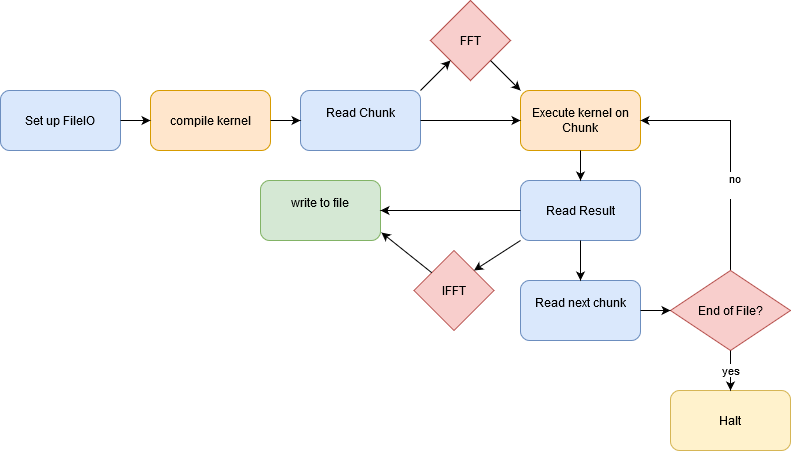
\includegraphics[width=\linewidth]{host1.png}
	\label{fig:host1}
\end{figure}

.

Some initial code based off https://www.eriksmistad.no/getting-started-with-opencl-and-gpu-computing/

\subsection{Sequential implementation}

We started exploring the problem by doing a simple 1d convolution in the time domain, this would allow us to verify values and serve as a guide to the general structure of the project.

\subsection{Parallel implementation}

\subsubsection{Kernels}

The time convolution kernel uses SPMD where each execution will attain an id and use that to execute the program, each execution will do one execution of the inner loop. I.E. for the ith input in the signal we calculate that value by executing the inner loop, looping over the elements in the FIR to get the value in the convolution corresponding to that ith value in the input signal. This kernel is given chunks until there is no more file left, and the results are all written.

\begin{figure}[!htb]
	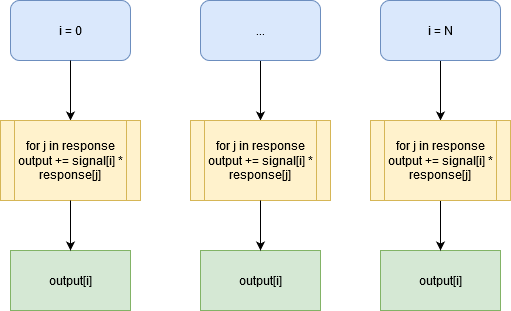
\includegraphics[width=\linewidth]{host2.png}
	\label{fig:host2}
\end{figure}

.

\subsubsection{Time domain specifics}

For the implementation for the GPU time convolution the host code builds the time convolution kernel  then runs it with chunks it fetches from the file we are processing. Chunks of the file are fed to the kernels and written to disk by a separate thread while the next chunk is read in.

\subsubsection{FFT}

We encountered run time speed issues with VexCL as the fft should not really take that long, it currently takes longer to do our overlap save than time convolution. This is likely the current bottleneck for overlap save.

\subsubsection{Performance}

Time convolution is 28x faster than overlap save, run times were 2765ms and 77723ms. This was performed on a data set containing a signal input size of 1,000,000 values and a filter of length 64.

\subsection{Overlap save implementation}

Our project required us to perform signal filtering on a large amount of signal data or with a large filter size. So our group decided to process signal data in the frequency domain and so we used a discrete fourier transform library to perform the fast Fourier transform algorithm (FFT). The reason for performing the transformation with FFT is we can use an algorithm called overlap save which is excellent at filtering signal input efficiently by employing data chunking. The filter used is a finite impulse response filter which filters the signals impulse response in a finite amount of time (signal decays or stops, reaching 0). 

In the GitHub project, Overlap save is implemented sequentially under \begin{verbatim}project\CpuSequential\convolution_in_opencl\cpu_sequential\end{verbatim} and parallel implementation is under \begin{verbatim} project\OpenCL\opencl_base\OverlapSave.h \end{verbatim}

\subsubsection{Sequential implementation}

Sequential implementation takes a given CSV file containing the time, filter coefficients and signal data which it then processes and passes the required information to the overlap save algorithm. 

First, Overlap save takes a  block of the data dependent on the size of the filter used, using a minimisation cost function to determine the block size, the size is influenced by the size of the filter such that when FFT is performed, it requires the least amount of complex multiplications to perform the total filtering.

The length of the total signal data is found and is needed to end the while loop to stop processing new blocks when it reaches the end of the data. The size of the filter is also found, this is needed because we need to find the overlap in each block of data. Since overlap save is performing FFT/multiplication and data transforming in blocks, the algorithm can be easily parallelised. The difficulty with this is that for the blocks to smoothly flow on from one another, there must be some overlap of signal data from the end of the previous block at the start of the current block. This overlap means the results from each block when stitched back into order, will return the same result as if filtering and convolution has occurred all at once, int overlap = m - 1 is set which tells the algorithm that the amount of overlapped values in each block is equal to the length of the filter - 1. We also find the step size of each block, the step size of the amount of new input we need to read minus the padded values. We use step size to increment a position counter so that we can keep track of how much unique signal data we have processed and where to start reading from the file/chunk to get the next block of data.

For complex FFTW and complex multiplication to return the correct frequency values we pad by adding 0s on the end such that the filter has the same length as the size of the block. Padding must also be added to the first and last blocks of data, the first block is padded on the start with the length of the overlap in 0s and the same is done on the last block except the 0 padding occurs at the end of the block. This keeps all the block lengths uniform and insures all the signal data is processed. Every block in between the first and the last has an overlap of the previous blocks end data (of size overlap) to meet the above output correctness.

So while the position plus the size of the block is less than the total length of the data we know there is still signal values needing to be processed. We first pre compute the filter FFT as this will be used in every iteration of the while loop for complex multiplication and will be wasteful to recompute on every new block iteration. Now in the while loop we first take a vector of the signal data between the position index and the position plus the block length. FFT is then performed on this vector and its complex output is multiplied with the filters complex FFT output. Finally the output from the multiplication is inverse FFT which returns the filtered signal array. This filtered signal still contains the overlapped data we were using to compute the start of the FFT so block results would naturally flow consistently as mentioned above. This extra data is not needed any more and these added values are not part of the complete filtered end result so only the values between the position plus step size index and the position plus block size are saved in the final frequency vector.

Lastly the position value is incremented by the step size, this value is not incremented by the full block size as remember each block requires padding. Having the position be set smaller means that when the vector of signal data is found it will contain some of the previous blocks data as overlap.

\begin{figure}[!htb]
	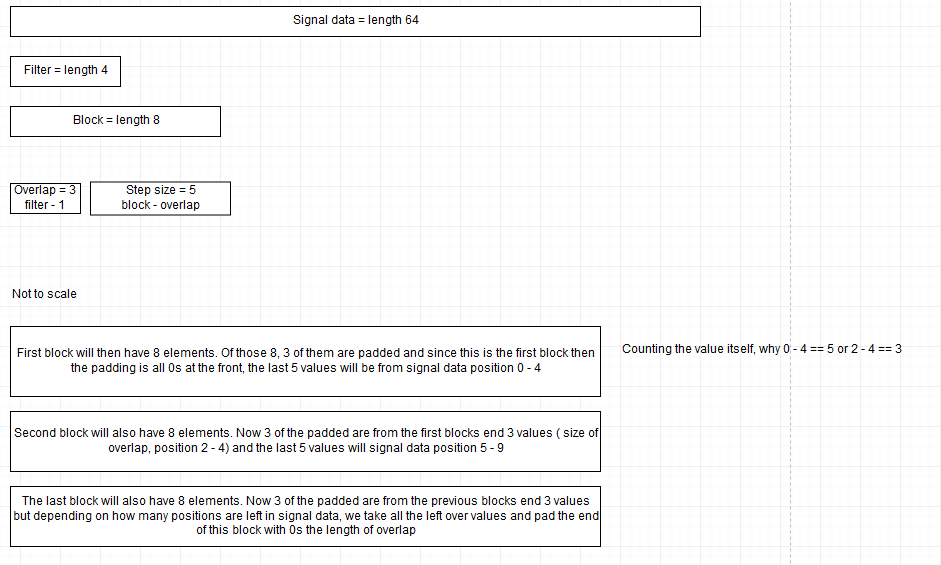
\includegraphics[width=\linewidth]{example1.png}
	\caption{Example implementation of block structure in overlap save}
	\label{fig:results1}
\end{figure}

Performs FFT on the filter and for each block of data, performs FFT on the block and does a complex multiplication between the FFT of the filter and the FFT of the data. This result is then inversed FFT and the required data from each block is returned as the filtered data. This is a high level overview and I will go into more depth during the sequential implementation explanation.

\subsubsection{Parallel implementation}

The parallel implementation is very similar to the sequential implementation bar some key differences. Our implementation uses the OpenCL Nvidia SDK libraries 

Chunking and data reading is done by the groups written I/O functions and so padding does not have to be added only accounted for as we still need to remember the position of the next new chunk of data.

Instead of FFTW, VexCl is used so we need to setup the kernel. VexCl will run the FFT on a separate OpenCl kernel so it can take advantage of the parallel computing on the GPU.

We also pass the complex multiplication off to be done in an OpenCl kernel to also take advantage of parallelisation. We set the kernels item size to be the same size as the length of the block. Since there is a multiplication done between each value/complex number between the filter FFT and the signal data FFT, we can tell the kernel to do every single multiplication separately in a new kernel so that we can run all the multiplications in parallel. 

Lastly we have the results of all the computed frequencies written to a file in a sequential fashion so we dont have any race conditions and we still remove the unneeded overlap.

The main difference between the sequential and the parallel implementation is we take advantage of being able to compute each FFT step and the complex multiplication in parallel so on very large blocks and sections of file read into ram we take advantage of the parallelisation possible.

\section{Results}

\subsection{Memory IO Results}

\begin{figure}[!htb]
	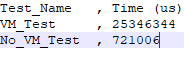
\includegraphics[width=\linewidth]{results1.png}
	\caption{A) Shows the amount of time taken to retrieve and process all chunks so that they are ready to be sent off to the GPU.}
	\label{fig:results1}
\end{figure}

From figure 3 we can see that my implementation is 35x less efficient than the standard ifstream implementation provided by the C++ library.

\section{Evaluation}

\subsection{Input bottleneck}

After having tested how well my proposed implementation fares against the standard ifstream provided to us by the C++ library I have found that I was incorrect in my assumption that my implementation would be faster than the C++ library. This would imply that ifstream already accounts for having to read large data files.

As my implementation is slower than what is provided by the standard C++ library we will need to find a different method of loading large datasets into our project in the future. I propose two methods as a potential solution. 

The first method is a multithreaded version of the current memory mapped implementation. In this method we would load the data into a virtual address space again, however instead of reading data using only a single thread we would instead use multiple threads. Each thread would produce a chunk of data that would be sent off to the acceleration unit. 

The second method is to use the new shared virtual memory feature implemented in openCL 2.0 to allow the acceleration unit to grab the data it needs from the file without needing the host code to load the data into RAM first. This is achieved using the “cl SVM alloc” function, which is a shared virtual memory function that allows a pointer to be shared between the host and the device \cite{mccardwell2015fir}.

\subsection{Memory management}

Our future time would be spent on optimisation of parameters as well as balancing the amount of time spent in file reading and copying values between different containers, unfortunately not having a standard container across the entire project has mean many conversions, luckily in type system such as C++ this is fairly painless as you are quite sure of what types you are dealing with but it is very easy to change between them, compared to Java where casting can be very rigid, and compared to a dynamically typed language where you are never quite sure.

We have unfortunately not optimised for cache or ram currently. This means we are likely suffering from a lot of very timely ram and cache misses, we have very poor memory efficiency as well. This program uses about twice the file size in ram. Improvements to this would be in structuring our data better and performing less copies, trying to use a few containers as possible.

\subsection{OpenMP usage}

We would also like to improve the amount of parallel processing the host code, future work using OpenMP std::threads more often that we did.

\subsection{Don't over complicate}

Building on using more high level features looking into the C++ bindings for OpenCL would be a good improvement for this project unless there is a tangible performance hit, as we ended up wrapping many calls directly to the C api anyway. There were instances where standard libraries would have done an efficient job at completing some jobs but were overlooked for more complicated solutions like reading and writing files.

\subsection{Communicate more and follow a group coding structure}

Challenges trying to write good API for specific reading/chunking operations, where we want to support different padding options but not having to pad explicitly in the files that handle calling kernels as this makes for very unreadable code. It took hard work and communication to get areas of code that interfaced across all three of us to work as intended for a wide variety of uses. We found that OpenCL lacked some built in functionality that one would get from other frameworks or as well supported and documented libraries.

\subsection{Future work on finding optimal kernel size}

We also often encountered challenges with the work group item sizes (for kernels) quite often results would be completely blank due to value being incompatible with each other. We would like to have a way to select optimal sizes for this in future to minimise the waste of resources.

\subsection{Implement our own FFT algorithm}

FFT adds a lot to our runtime currently and we would like to improve that greatly in future. We do not know how to tune the performance of VexCL and it was mainly chosen as an easy way to get the FFT step onto the GPU but in hindsight it probably would have been faster to switch back to using FFTW in the host code. Ideally, we would implement our own FFT or port FFTW to a kernel or some of its execution).  Theoretically FFT should help us as the inputs get larger but unfortunately, we could not test to this point as our runtimes were getting so large even on release configuration builds that it is very unlikely the overlap save implementation would ever catch up. The large the FIR array/kernel the faster we would expect to see overlap save get to the time domain.

\subsection{Optimise chunk size}

Minimisation function was not fully implemented so we were asking the user to provide the correct or their desired block size which may cause efficiency problems if this value is poorly choosen.

\subsection{Chunking to small, wasteful I/O}

We were chunking the data, reading chunks into RAM but then grabbing chunks the same size as what blocks were going to be set as. This is really inefficient and meant every since cycle of overlap save we were having to read another block/chunk from disk. Considering overlap save requires more overall chunk computation due to overlap (takes longer to cycle through the complete data). This means compared to time convolution which has fewer reads, overlap save takes a massive hit. Saturating the RAM/VRAM and reading in blocks then writing to a file will greatly minimise the amounts of reads as new data only has to be read once the saturated RAM has been fully worked on/read.

\section{Work done}

\subsection{Jeremy Lang}
OpenCL setup/boilerplate, sequential time convolution implementation, Vex/FFTW setup/boiler, complex opencl kernel, reading/writing wrappers, benchmarking

\subsection{Reuben Speirs}
Sequential and parallel overlap save implementation, benchmarking, latex report setup

\subsection{Victor Startsev}
Matlab data visualisation, data generation, reading/wrinting data to and from file/CSV

\bibliographystyle{plain}
\bibliography{Bibliography}
\nocite{*}
\end{document}